\chapter{Baza de date}

În acest capitol este argumentată alegerea unui tip de baze de date SQL, mai exact MySQL, pentru a reține informații importante aplicației. A fost preferată o abordare clasică asupra unei baze de date relaționale în special datorită numărului mare de tranzacții ce necesită o asigurare mai mare a integrității datelor \cite{sql1}.

Aplicația \thesistitle este de tip utilitar, aceasta are scopul de a fi folosită într-un context restrâns, în cadrul facultății. Prin urmare numărul de utilizatori este unul relativ mic, reprezentat de către studenți și profesori. De asemenea, poate fi observată o relație strânsă între profesori și propunerile acestora, dar și între studenți și preferințele acestora.

Relațiile între entități sunt de mai multe tipuri, în special \textit{One-to-one} și \textit{One-to-many}. Acest lucru se poate observa în diagrama următoare a bazei de date utilizate.

\begin{figure}[H]
	\centering
	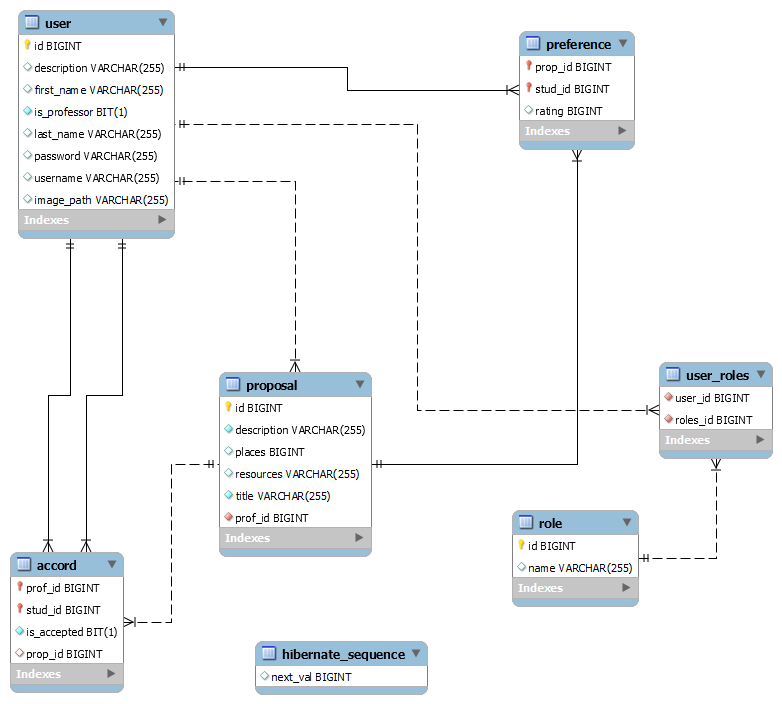
\includegraphics[width=\textwidth, left]{DB_diagram.png}
	\caption{Baza de date}
\end{figure}

În următoarele subcapitole sunt detaliate modelele utilizate pentru a reprezenta aceste date.

\section{Modelarea utilizatorilor}

Utilizatorii au fost modelați într-un mod clasic. Aceștia au la rândul lor roluri în funcție de drepturile pe care le au ei în cadrul aplicației. Astfel, sunt identificate două astfel de roluri: \textbf{ROLE\_USER} și \textbf{ROLE\_ADMIN}. Pe lângă acest lucru, utilizatorii sunt ori profesori, ori studenți, particularitate ilustrată de câmpul boolean \textit{is\_professor} al entității \textbf{\texttt{user}}.

\begin{figure}[H]
	\centering
	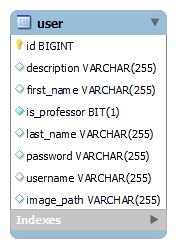
\includegraphics[width=0.3\textwidth, center]{user_model.png}
	\caption{User}
\end{figure}

Fiecare utilizator este identificat unic printr-un \texttt{id} de tipul de date BIGINT, care este și cheie primară a entității. Ca în majoritatea cazurilor, aceștia au un nume de familie (\texttt{last\_name}) și un prenume (\texttt{first\_name}). Câmpul \texttt{username} este de tipul VARCHAR(255) și este reprezentat de un email valid, lucru asigurată pe partea de front-end. Câmpul \texttt{password} este tot de tipul VARCHAR(255) și reprezintă parola utilizatorului, însă criptată pe partea de back-end cu un algoritm clasic.
Aceste două câmpuri sunt primite de către utilizator din partea unui administrator și sunt utilizate pentru autentificarea în aplicație. A fost preferată această abordare pentru a împiedica crearea de conturi din partea unor persoane din afara contextului.

\subsection{ROLE\_USER}

Cei mai mulți utilizatori au rolul \textbf{ROLE\_USER}, un rol default. Acest lucru le autorizează accesul la aplicație, odată ce aceștia sunt autentificați. Interfața diferă în funcție de tipul utilizatorului.

\subsubsection{Tipuri}

\textbf{Profesorii} pot crea și actualiza propuneri (en. proposals) pentru teza de licență. Aceste propuneri pot fi \textit{project} sau \textit{topic}, detalierea acestora urmând a fi făcută ulterior. De asemenea, aceștia pot încheia acorduri (en. accords) cu anumiți studenți pentru unele dintre propunerile lor. Acest lucru le permite studenților să nu mai participe la algoritmul de stable matching, fiind deja repartizați profesorilor respectivi.

\textbf{Studenții} pot crea și actualiza preferințe (en. preferences) într-o anumită ierarhie a lor. Așadar, categorisirea utilizatorilor în profesori și studenți are unicul scop de a diferenția interfața în funcție de funcționalitățile specifice tipurilor acestora.


\subsection{ROLE\_ADMIN}

Există în plus un număr restrâns de utilizatori care au rolul de administrator, \textbf{ROLE\_ADMIN}. Aceștia au dreptul de a gestiona conturile participanților, mai precis de a crea, actualiza și elimina utilizatorilor. De asemenea, administratorii au opțiunea de a impune anumite limite în cadrul aplicației cum ar fi o limită a propunerilor pentru profesori și o limită a preferințelor pentru elevi.

\section{Preferințele}

Preferințele sunt modelate simplu, reprezentând în sine o relație între entitățile studenți și propuneri.

\begin{figure}[H]
	\centering
	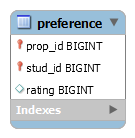
\includegraphics[width=0.3\textwidth, center]{preference_model.png}
	\caption{Preference}
\end{figure}

După cum se poate observa în tabela \textbf{\texttt{preference}}, acestea cuprind un \texttt{id\_stud} ce face legătura cu tabela \textbf{\texttt{student}} și un \texttt{id\_prop} ce face legătura cu tabela \textbf{\texttt{proposals}}.

În plus, există un câmp \texttt{rating} care este de tipul BIGINT și indică invers proporțional importanța preferinței, mai exact o preferință cu un $\texttt{level} = 0 $ este pe primul loc în ierarhie. Este de asemenea important de precizat că mai multe preferințe ale unui student pot avea același rating, lucru necesar pentru un algoritm de \textit{stable matching with ties}.

Aceste relații între studenți și tezele propuse vor constitui datele de intrare pentru algoritm, fiind astfel de o importanță semnificativă în cadrul aplicației.

\section{Propunerile}

În cazul propunerilor, la nivel teoretic acestea pot fi de două tipuri, proiect (en. project) sau temă (en. topic). Diferența constă în faptul că un proiect este o propunere mai concisă, cu o descriere exactă a lucrării așteptate, fie ea una de cercetare sau o aplicație propriu-zisă, iar un proiect nu poate fi ales și realizat decât de către o singură persoană.
Un astfel de exemplu ar putea fi \textit{„Realizare unei aplicații de reconoaștere facială utilizând metode de machine learning”}, cu precizările și restricțiile aferente.

Pe de altă parte, o temă este o descriere pe larg a anumitor particularități ale unui proiect de cele mai multe ori dintr-un anumit domeniu de specialitate. La fel ca un proiect specific, o temă poate cuprinde atât lucrări general teoretice, cât și practice, studentul fiind nevoit să stabilească împreună cu profesorul său coordonator o teză concretă. Însă o propunere de acest fel poate avea un număr de locuri disponibile mai mare de 1, deoarece mai mulți studenți pot urma direcții diferite asupra tematicii propuse. Spre exemplu, profesorul poate propune o temă de „Algoritmi genetici și optimizarea acestora” care poate fi repartizată unor 3 studenți care stabilesc în mod distinct cu profesorul de licență lucrările lor.

Cu toate acestea, din motive de simplificare și optimizare, la nivelul de scehmei de baze de date, a preferată modelarea propunerilor într-o singură tabelă intitulată sugestiv \textbf{\texttt{proposal}}, diferența dintre cele două tipuri fiind făcută de câmpul \texttt{places}. 

\begin{figure}[H]
	\centering
	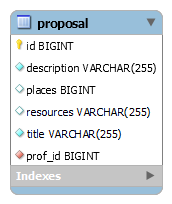
\includegraphics[width=0.3\textwidth, center]{proposal_model.png}
	\caption{Proposal}
\end{figure}

În cazul proiectelor (projects) câmpul acesta rămâne \texttt{null}, spre deosebire de teme (topics). Fiecare propunere are un titlu (\texttt{title}) reprezentativ și o descriere (\texttt{description}) adecvată de tipul VARCHAR(255), precum și o listă de referințe pentru a ajuta studentul. Ultimul câmp este \texttt{id\_prof} care indică autorul propunerii.


\section{Acordurile}

În cadrul aplicației \thesistitle, fiecare profesor poate stabili împreună cu un student un acord, reprezentat de tabela cu același nume \textbf{\texttt{accord}}, în ideea că acest student și propunerea aleasă nu mai sunt luate în calcul la rularea algoritmului de repartizare. Cu alte cuvinte, acest detaliu le permite studenților posibilitatea să realizeze un proiect preferat, adecvat abilităților și înclinațiilor sale, desigur cu aprobarea profesorului corespunzător tezei alese.

\begin{figure}[H]
	\centering
	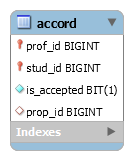
\includegraphics[width=0.3\textwidth, center]{accord_model.png}
	\caption{Accord}
\end{figure}

\section{Lucrul pe partea de back-end cu baza de date}

Partea de back-end a aplicației, fiind implementată cu ajutorul Spring Boot, interacționează cu baza de date prin intermediu Hibernate, alegere făcută luând în considerare o serie de avantaje.

\subsection{Hibernate}

\begin{figure}[H]
	
\includegraphics[width=0.3\textwidth, left]{hibernate-logo.png}
	\caption{\url{https://hibernate.org/images/hibernate-logo.svg}}
\end{figure}

\subsubsection{Ce este Hibernate}

Hibernate este un framework, mai precis un ORM (object relational mapping) creat pentru a facilita maparea modelelor orientate-obiect la baze de date relaționale pentru aplicații web \cite{hibernate1}. În mod intern, acest ORM utilizează JDBC API pentru a interacționa cu baza de date \cite{hibernate2}.

\begin{figure}[H]
	\centering
	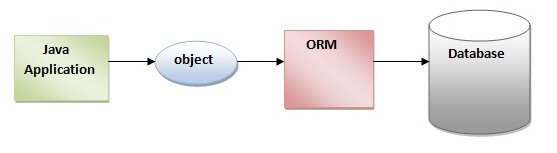
\includegraphics[width=0.3\textwidth, center]{orm.jpg}
	\caption{ORM}
\end{figure}

Hibernate este cu alte cuvinte o implementare a specificațiilor JPA (Java Persistence API) pentru persistența datelor. JPA este un set de reguli care oferă un standard definit și o anumită funcționalitate acestor tehnologii ORM \cite{hibernate2}.

\subsubsection{Funcționalitatea Hibernate}

Framework-ul precizat corelează clase din limbajul Java tabelelor din serverul de baze de date, dar și tipurile de date din Java cu cele din SQL pentru a asigura persistența obiectelor. Hibernate returnează astfel aplicației enitățile sub formă de obiecte Java și reduce astfel timpul de procesare a rezultatelor și codul necesar implementat de programator.

\subsubsection{Avantaje ale Hibernate}

Hibernate este în primul rând un framework \textit{open source} și \textit{lightweight}, lucru ce mi-a permis familiarizare cu acesta și ușoara configurare a lui.

În al doilea rând, Hibernate este un framework relativ rapid deoarece beneficiază de un cache intern, structurat pe două niveluri, primul nivel fiind folosit în mod normal \cite{hibernate2}.

De asemenea, tehnologia optată utilizează o versiune orientată obiect a SQL-ului, HQL (Hibernate Query Language), care permite generează query-uri independente de baza de date, fără a scrie în mod explicit query-uri în SQL \cite{hibernate2}.

În final, Hibernate oferă posibilitatea de a crea și popula tabelele din baza de date în mod automat, direct din cod.

Imaginea următoare ilustrează specificațiile din fișierul \texttt{application.properties} specific oricărui proiect Maven, în care sunt este configurată utilizarea framework-ului Hibernate. Acest lucru include date de conectare la baza de date, modul de conectare, dialectul SQL folosit etc.

\begin{figure}[H]
	\centering
	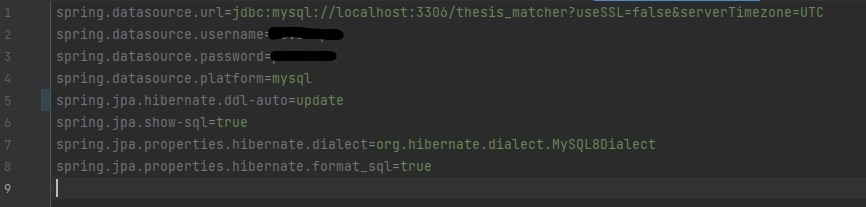
\includegraphics[width=\textwidth, left]{application-properties.jpg}
	\caption{application.properties}
\end{figure}

Pentru a putea folosi Hibernate într-un proiect de Spring Boot este necesară adăugarea dependenței următoare în fișierul \texttt{pom.xml}.

\begin{figure}[H]
	\centering
	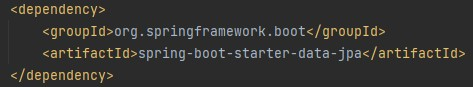
\includegraphics[width=\textwidth, left]{hibernate-dependency.jpg}
	\caption{Dependența din pom.xml}
\end{figure}

\section{Generarea datelor}

În vederea generării unor date reprezentative problemei actuale, a fost creată o clasă separată numită \texttt{Populator} ce introduce înregistrări (records) în baza de date. De aceea au fost stabilite în primul rând o serie de parametri care reglează dimensiunile populațiilor și proporțiile dintre diferitele tipuri de entități. În continuare vor fi prezentați pe scurt acești parametri și configurarea lor, urmând a descrie maniera de generare propriu-zisă a utilizatorilor, propunerilor profesorilor și nu în ultimul rând, preferințelor studenților.

Configurarea parametrilor necesari generării datelor este realizată prin intermediul unei clase \texttt{PopulatingConfiguration}.

\begin{figure}[H]
	\centering
	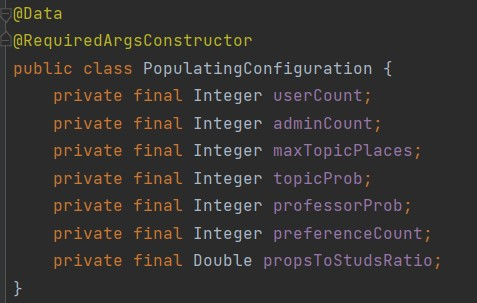
\includegraphics[width=0.6\textwidth, center]{populating-config-class.jpg}
	\caption{Clasa de parametri de configurare}
\end{figure}

Aceasta conține parametri precum numărul de utilizatori (\texttt{userCount}), numărul de administratori (\texttt{adminCount}), probabilitatea ca un utilizator să fie profesor 
(\texttt{professorProb}) etc.

Primul pas este generarea utilizatorilor. Pentru această etapă a fost folosită clasa \texttt{Faker} în obținerea unor nume aleatorii. Parola tuturor a fost setată aceeași pentru simplificare, iar primi \texttt{adminCount} utilizatori primesc \texttt{ROLE\_ADMIN} pe lângă \texttt{ROLE\_USER}.

Cel de al doilea pas este generarea propunerilor pentru fiecare profesor ales dintre utilizatori conform unei probabilități. Se calculează întâi un număr de locuri în corelație cu numărul de studenți ce trebuie acoperit de fiecare profesor pentru a putea da șansa unei repartizări a tuturor studenților. De menționat că tipul propunerilor este tot ales aleatoriu.

Ultimul pas este crearea preferințelor și a acordurilor utilizatorilor.

În cazul de față, numărul total de utilizatori a fost ales \textbf{500}, cu o probabilitate de \textbf{10\%} ca un utilizator să fie profesor. Fiecare student are \textbf{20} de preferințe, iar numărul total de propuneri este într-un raport de \textbf{1.2} cu numărul total de studenți.